\documentclass{article}
\usepackage[top=1in,bottom=1in,left=1in,right=1in]{geometry}
\usepackage{graphicx}

\begin{document}

\section*{Hardware Requirements}
\paragraph*{}
The hardware portion of this project is divided into two portions, one set of nodes designed for reception and position estimation of a mobile signal, and one mobile node which will be responsible for broadcasting information gathered from the sensor. Each receiving node will consist of a MiWi device, an antenna, and possibly a microcontroller to handle sending of data. Each mobile node will connect to the primary ARM board, and transmit the data they received to it for further processing. The ARM board will be responsible for calculating the mobile unit's position, and logging the sensor data transmitted by it to an SD card attached to the device. It will also be responsible for displaying the sensor data on the attached LCD, as well as hosting the webserver which will provide an expanded view of the logged data. As a whole, the receiving segment will consist of at least 4 receiving antennas and the ARM board.

On the transmitting unit's side, there will be one MiWi board responsible for sending the sensor data, and a microcontroller with a sensor which will provide the data to be transmitted. The sensor in this case will be a GPS Reciever, which will provide location data to be compared against the position calculated by the analysis of the signal.

\section*{OS and Systems Software Requirements}
\paragraph*{}
For the ARM based base station to function properly, a number of services from
the operating system will be required.  To use the MiWi devices for distance
measurement, we will need to directly access the controller to view the RSS of
receive frames.

In order to write log data to an SD card, we will need both a means to write raw
blocks to the SD card as well as a filesystem to organize the data in a way that
we can easily read/write with a portable computer. 

To transfer data too and from the wireless nodes, we will need an $I^2C$ driver,
since all of the nodes will be on such a bus.  Such a driver will need to
implement master mode and be able to read data from any of the slave nodes.  To
manage threads/contexts for all of the devices being operated, we will use
FreeRTOS's lightweight threads, and the message passing interface that it
implements.

\section*{Radio requirements}
\paragraph*{}
The ultimate goal of this project is to estimate position using a 2.4 GHz MiWi system.  Within the scope of this project are two viable methods by which position estimation can be performed.  The first of these is \textit{Received Signal Strength}.  Over a given sample period data would accumulate from each receiver node.  Whereupon, the ARM board will compute a certain confidence interval for transmitter range (using free space path loss assumptions, or some type of ricean fading distribution), the end result would be an overlap area for the most likely location of the transmitter.  The second method is a type of \textit{Space Analysis} where measurements are taken in a predetermined grid to establish the RF environment.  The computations required to establish position are much more complex and involve an algorthim resembling:
\begin{equation}
D_{i} = \vert R_{i} - \sqrt{ \left( x' - x_{i} \right)^{2} +\left( y' - y_{i} \right)^{2} } \vert
\end{equation}
\paragraph*{}The optimization function becomes:
\begin{equation}
\phi\left(x,y\right) = \sum_{i=0}^{2}D_{i}
\end{equation}
\paragraph*{}This function is generally concave, therefore we can take the gradient of it and add a step to follow this function to its minimum.
\begin{equation}
\left(x_{next},y_{next}\right) = (x,y) + \nabla\phi\left(x,y\right)\cdot stepsize
\end{equation}
\begin{equation}
\nabla\phi = \frac{\delta}{\delta x}\phi\left(x,y\right)\hat{x} + \frac{\delta}{\delta y}\phi\left(x,y\right)\hat{y}
\end{equation}
\paragraph*{}To simplify this for embedded system calculations, we approximate the magnitude function with a squaring operation and define the below equations.
\begin{equation}
K_{i} = \sqrt{\left(x-x_{i}\right)^{2} + \left(y-y_{i}\right)^{2}}
\end{equation}
\begin{equation}
\nabla\phi\left(x,y\right) = \hat{x}2\left[\sum_{i=0}^{2}\left(R_{i}-K_{i}\right)\left(\frac{-1}{2K_{0}}\right)\left(-2x+2x_{i}\right)\right] + \hat{y}2\left[\sum_{i=0}^{2}\left(R_{i}-K_{i}\right)\left(\frac{-1}{2K_{i}}\right)\left(-2y+2y_{i}\right)\right]
\end{equation}

\section*{User Interface}
\paragraph*{}
The ARM board will receive data from the sensors on the MiWi board and write out all relevant values to a log file on an sdcard in comma-separated values (CSV) format. The data logged includes GPS coordinates, RSSI position data, clock/times, and other information to be determined that needs to be displayed. To display any data and calculations, we will utilize the LCD and provide a web page served through an ethernet connection available on the ARM board. Both methods of display are capable of navigation through user-input.

The web interface and the on-board LCD will give users a way to view the data in a meaningful format. The web page interface will display data and calculated values in a tabular format. The page will be created on-demand when a user accesses it with data that the ARM board holds in its logs at those times. The UI on the LCD will display the data in a similar table format row by row. Interaction with the LCD should either bring up more options or display other data.

\section*{Diagrams}
\subsection*{Drillfield node placement}
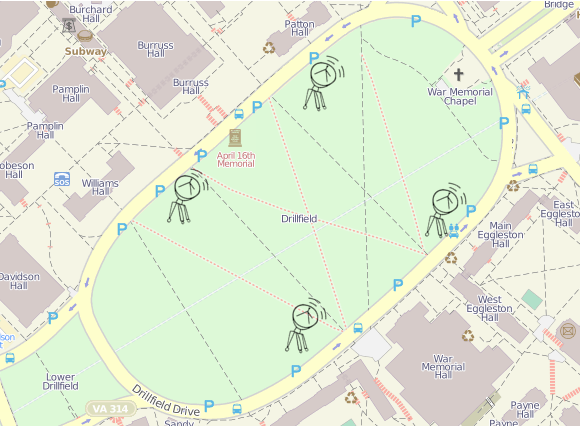
\includegraphics[width=0.5\textwidth]{node_placement}
\subsection*{System Diagram}
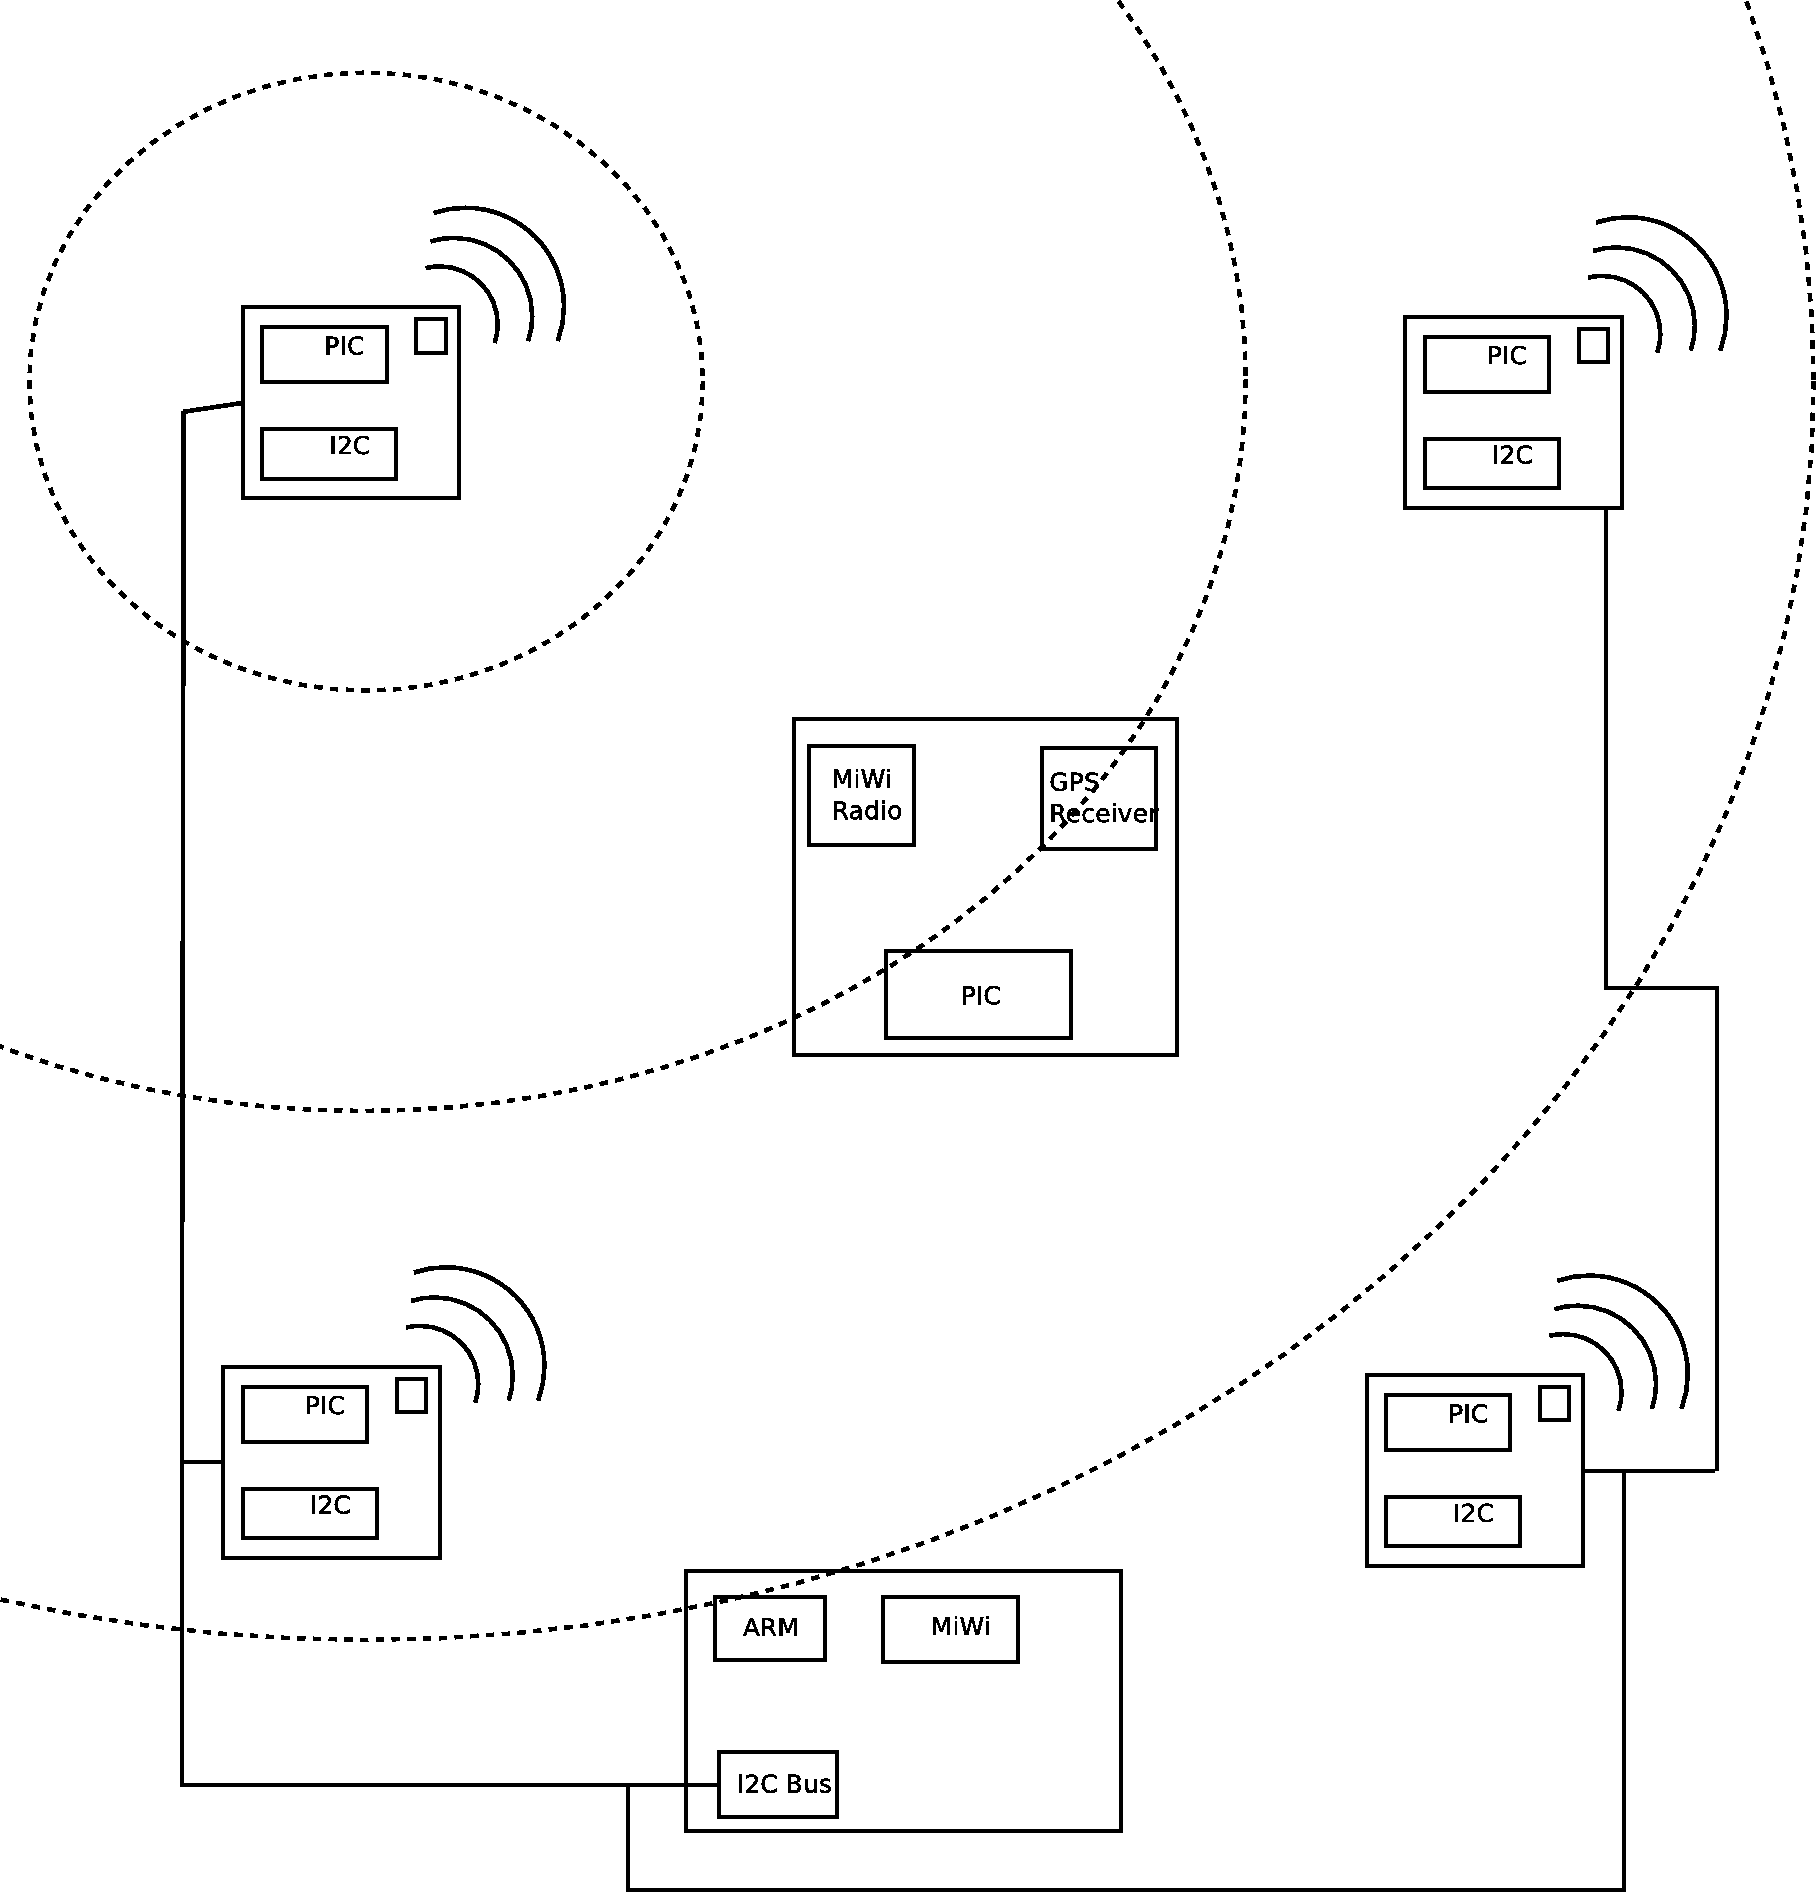
\includegraphics[width=0.5\textwidth]{system}

\end{document}
